%%%% Paramétrage du TD %%%%
\def\xxactivite{Révisions \ifprof -- Corrigé \else \fi} % \normalsize \vspace{-.4cm}
\def\xxauteur{\textsl{Xavier Pessoles}}


\def\xxnumchapitre{Révision 1 \vspace{.2cm}}
\def\xxchapitre{\hspace{.12cm} Résolution des problèmes de statique -- Statique 2D}
\def\xxonglet{\textsf{Rév -- Stat}}
\def\xxactivite{TD 01}
\def\xxauteur{\textsl{Xavier Pessoles}}

\def\xxpied{%
Révision statique -- Résolution des problèmes de statique plane\\
Fiche 1 -- \xxactivite%
}

\def\xxcompetences{%
\vspace{-.3cm}
\textsl{%
\textbf{Savoirs et compétences :}\\
%\vspace{-.4cm}
%\begin{itemize}[label=\ding{112},font=\color{ocre}] 
%%\item \textit{Res1.C4 : } Correction
% \item \textit{Res1.C4.SF1 : } Proposer la démarche de réglage d’un correcteur proportionnel
%%proportionnel intégral 
%%et à avance de phase
%\item \textit{Con.C2 : } 	Correction d’un système asservi	
%\item \textit{Con.C2.SF1 : } Choisir un type de correcteur adapté
%\end{itemize}
}}

\def\xxauteur{\textsl{Xavier Pessoles}}

\def\xxtitreexo{Modélisation du captage du courant dans un train à grande vitesse}
\def\xxsourceexo{\hspace{.2cm} \footnotesize{Concours CCINP 2018}}

\def\xxfigures{
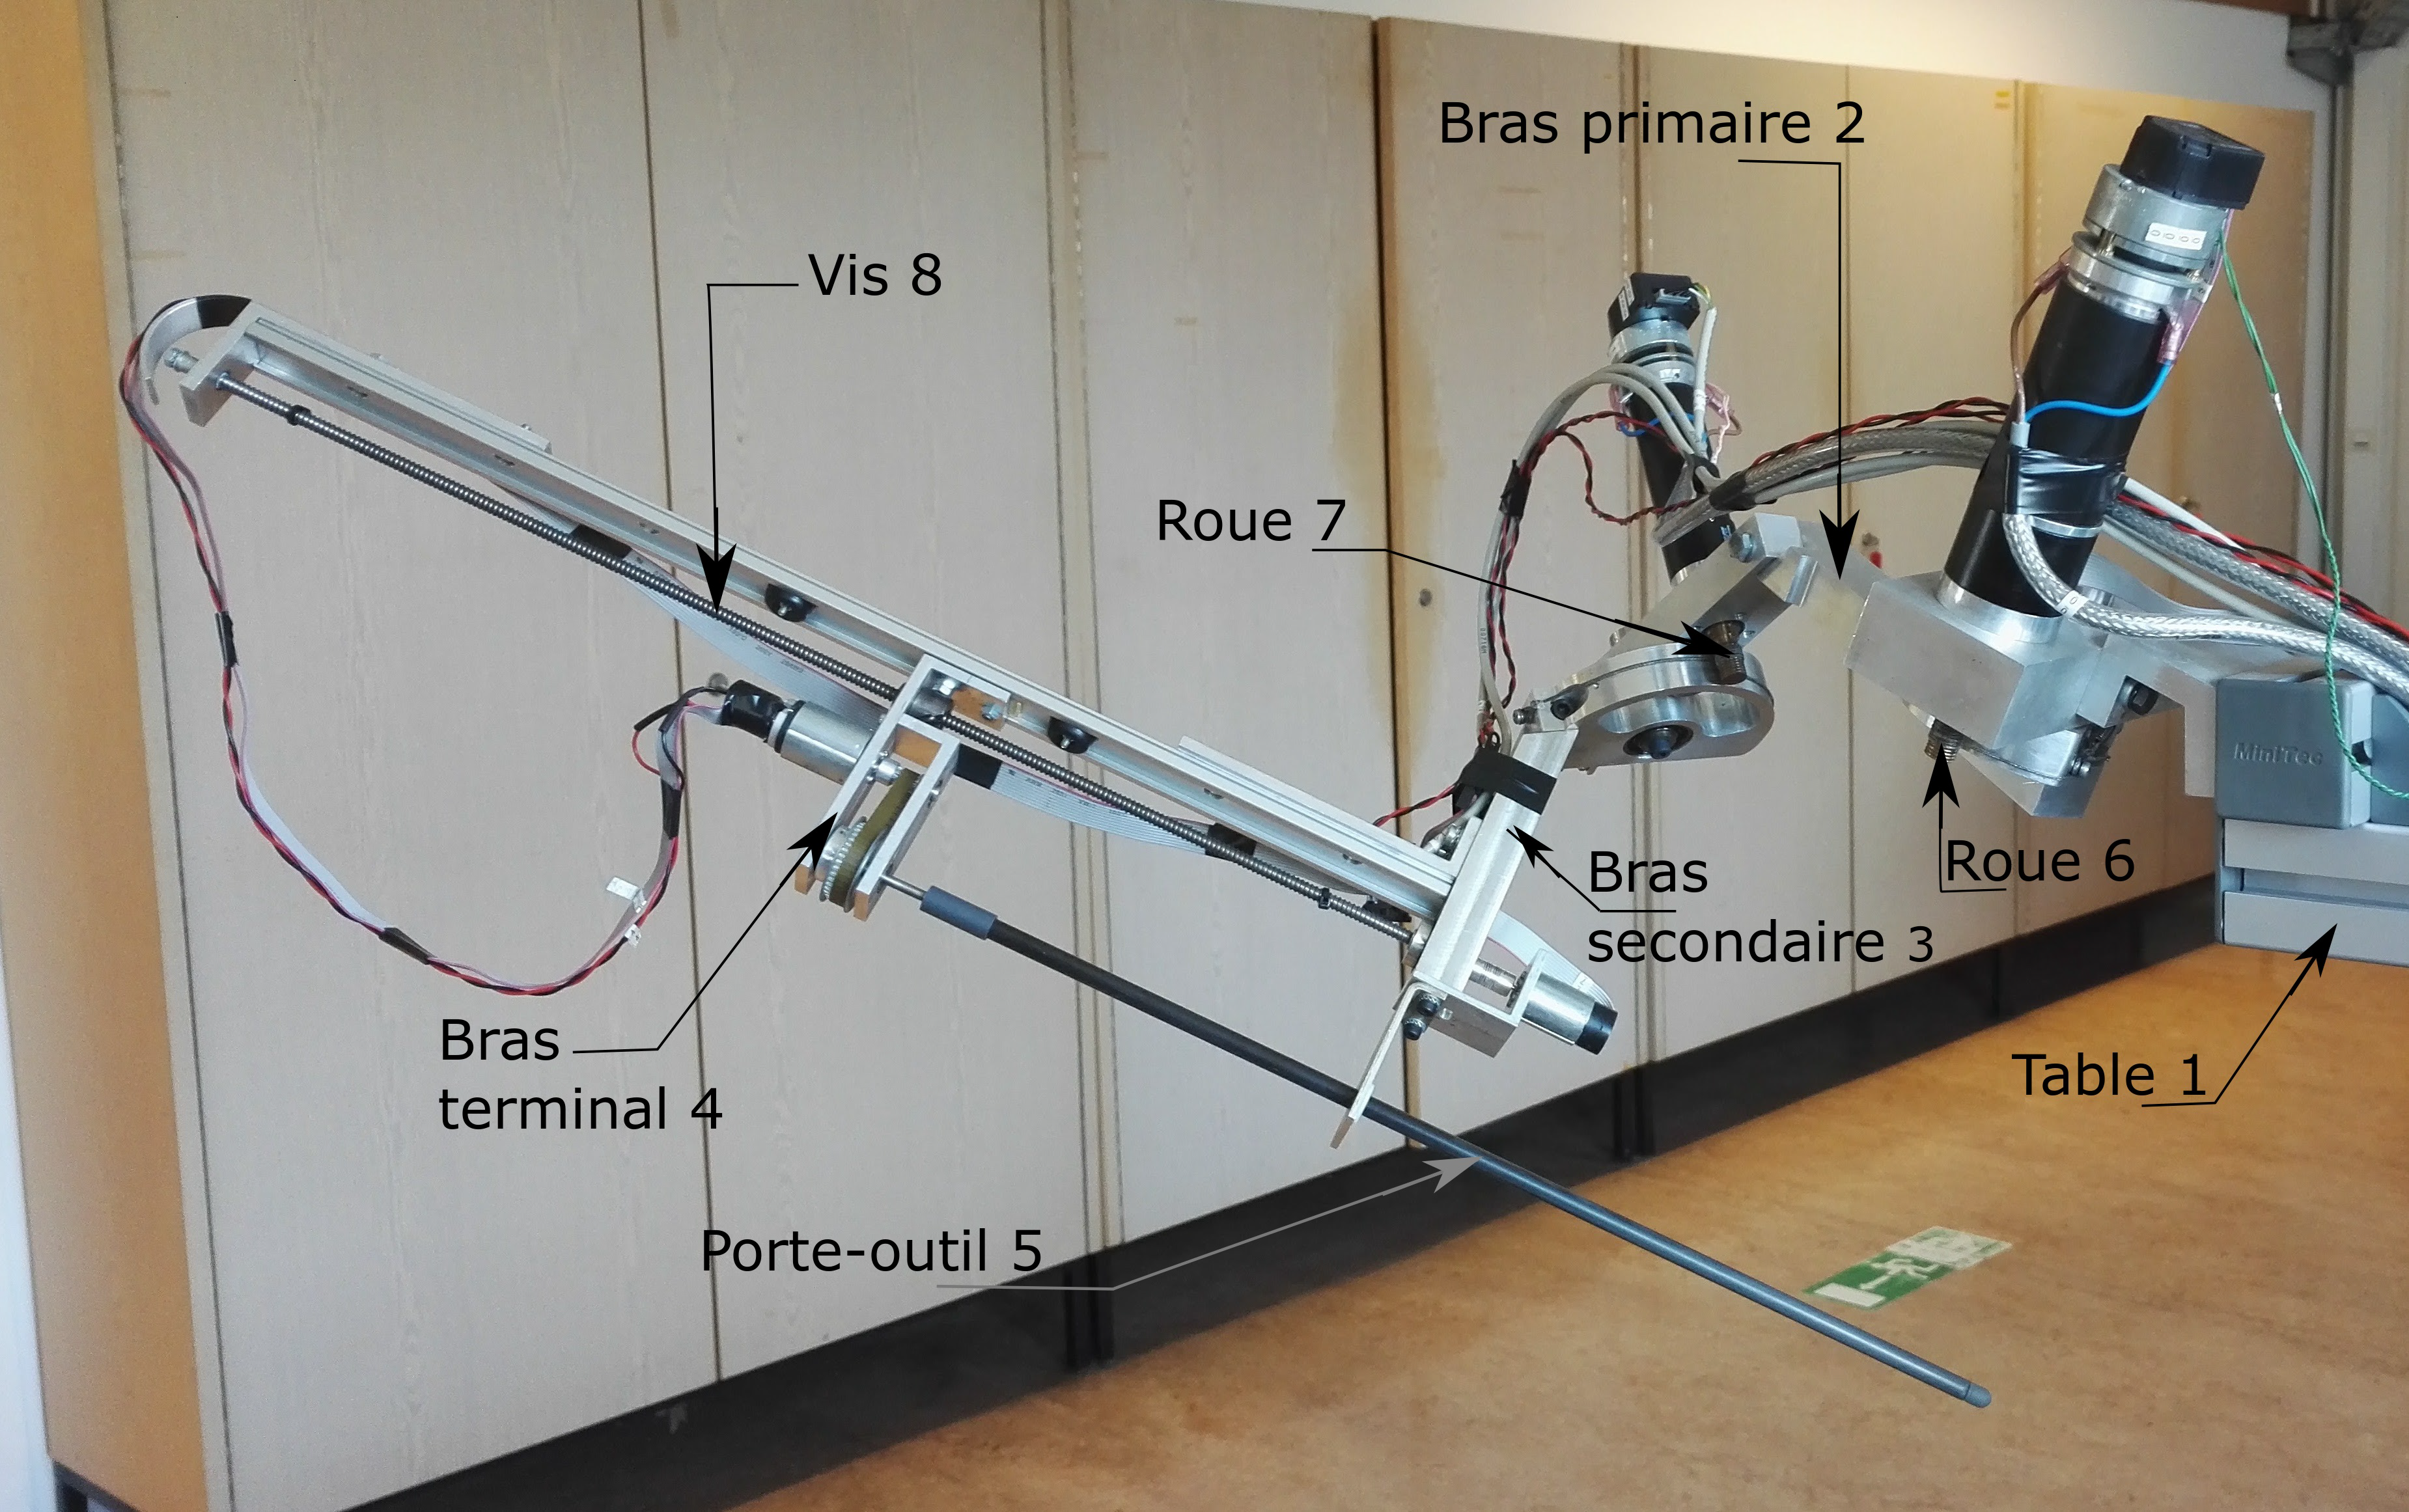
\includegraphics[width=.55\textwidth]{fig_00}
}%figues de la page de garde


\iflivret
\input{style/new_pagegarde}
\else
\input{style/new_pagegarde}
\fi
\setlength{\columnseprule}{.1pt}

\pagestyle{fancy}
\thispagestyle{plain}

\vspace{5cm}

\def\columnseprulecolor{\color{ocre}}
\setlength{\columnseprule}{0.4pt} 

\setcounter{exo}{0}

%\ifprof
%%\begin{multicols}{2}
%\else
%\begin{multicols}{2}
%\fi
%%%%%%%%%%%%%%%%%%%%%%%%%%%%%%%%%%%%%%%%%%%%%%%%%%

\section*{Présentation générale}
\section{Étude préliminaire de la ligne d'alimentation}
\subsection{Calcul des pertes dues à la caténaire}
\subparagraph{}

Dans le cycle de vie du produit, et notamment les phases d'entretien, il est préférable de changer le matériau de la bande de captage car il est plus facile (et moins coûteux) de changer cette pièce que tout le câble de la ligne grande vitesse. 

\subparagraph{}
Le graphite est d'une part un très bon conducteur. D'autre part il favorise le glissement entre les pièces. 
On peut retrouver des électrodes en graphite dans l’électro-érosion (processus de fabrication bien connu de tous ;)). 
On l'utilise aussi pour la réalisation des collecteurs des moteurs à courant continu (permettant d'exploiter les deux propriétés citées). On l'utilise aussi dans des solutions de joints (garniture mécanique) pour favoriser le glissement entre pièces.


\subparagraph{}
Les deux schémas ci-dessous étant équivalent, les deux résistances sont donc en parallèle et $R_e = \dfrac{R_1R_2}{R_1+R_2}$. 
Par ailleurs, on  a $R_1 = xr$ et $R_2 = \left(L-x\right)r$. On a donc  $R_e = \dfrac{xr\left(L-x\right)r}{xr+\left(L-x\right)r}$$= \dfrac{xr\left(L-x\right)}{L}$. 

\begin{center}
\includegraphics[width=.8\linewidth]{fig_01}
%\textit{}
\end{center}


\subparagraph{}
On a $R_e(x)= \dfrac{xr\left(L-x\right)}{L}$. En dérivant, 
$R_e'(x)= \dfrac{Lr-2rx}{L}$.$R_e'(x)=0 \Leftrightarrow \dfrac{Lr-2rx}{L} = 0 $ 
$ \Leftrightarrow L-2x = 0 $ $ \Leftrightarrow x = \dfrac{L}{2}$.
%\section*{Mise en situation}

\subparagraph{}
Dans ces conditions, $R_e = \dfrac{L/2r\left(L-L/2\right)}{L}$ $= \dfrac{rL}{4}=\SI{0,05}{\Omega}$


\subparagraph{}
Aux bornes de la résistance équivalente, on a $U_R = R_e I =0,05 \times 2,5 \times 10^3= \SI{125}{V}$.



\subparagraph{}
On définit le rendement comme $\eta = \dfrac{\mathcal{P}_{\text{motrice}}}{\mathcal{P}_{\text{Alimentation}}}$
$ = \dfrac{U_M I}{U I} = \dfrac{U-U_ {R_e}}{U}= \dfrac{U-I R_e}{U}$. 

D'où $\eta = \dfrac{1,5\times 10^3 - 2,5\times 10^3 \times 0,05}{1,5\times 10^3}$ $= \dfrac{1,5 - 2,5 \times 0,05}{1,5}=92\, \%$.
\begin{center}
\includegraphics[width=.3\linewidth]{fig_02}
%\textit{}
\end{center}

\subsection{Passage au \SI{25}{kV} alternatif}
\subparagraph{}
Utiliser une tension plus élevée permet de diminuer les pertes en ligne.

\subparagraph{}
La fréquence de \SI{50}{Hz} est celle distribuée par les producteurs/transporteurs/fournisseurs d'électricité. 
Pour passer de $\SI{63}{kV}$ à $\SI{50}{kV}$ il est nécessaire d'utiliser un transformateur.

\section{Modélisation thermique de la caténaire, train à l’arrêt}

\subsection{ Régime transitoire dans la zone $P_1$ : $- L_1 <z < -L_c /2$}

\subparagraph{}
On isole une tranche de câble (section $S=\pi R^2$, largeur $\dd z$).
Un flux est le produit d'un flux de densité thermique (surfacique) et d'une surface. On utilise la loi de Fourier et 
$\Phi(z,t)=-\lambda \dfrac{\partial T(z,t)}{\partial z}\pi R^2$.

\begin{itemize}
\item le flux entrant en $z$ est : $\Phi(z,t)=-\lambda \dfrac{\partial T(z,t)}{\partial z}\pi R^2$;
\item le flux sortant en $z+\dd z$ est : $\Phi(z+\dd z,t)=-\lambda \dfrac{\partial T(z+\dd z,t)}{\partial z}\pi R^2$;
\item le flux latéral : $\delta \Phi_{\text{latéral}}=h\left(T(z)-T_e \right)2\pi R \dd z$.
\end{itemize}
\subparagraph{}

\subparagraph{}

\subparagraph{}

\subparagraph{}

\subparagraph{}

\subparagraph{}

\subparagraph{}

\subparagraph{}

\subparagraph{}

\subparagraph{}


\subparagraph{}

\subparagraph{}

\subparagraph{}

\subparagraph{}

\subparagraph{}

\subparagraph{}

\subparagraph{}

\subparagraph{}

\subparagraph{}

\subparagraph{}

\subparagraph{}


\subparagraph{}

\subparagraph{}

\subparagraph{}

\subparagraph{}

\subparagraph{}

\subparagraph{}

\subparagraph{}

\subparagraph{}

\subparagraph{}

\subparagraph{}

\subparagraph{}


\subparagraph{}

\subparagraph{}

\subparagraph{}

\subparagraph{}

\subparagraph{}

\subparagraph{}

\subparagraph{}

\subparagraph{}
